\frame
{
\frametitle{\citetitle{MarcoNuno_CongArbIng_2009_06_00}}
\begin{columns}
    \column {0.75\textwidth}
\begin{itemize}    
\item Las Redes Neuronales Pulsantes (SNN) son tema de investigación relevante debido a la plausibilidad biológica mostrada por estos modelos. 
\item Un estudio comparativa acerca de implementaciones en FPGA de clásicos y pulsantes arrojó que estos últimos son menos voraces respecto al uso de hardware en compración con los modelos de segunda generación.
\item Dependiendo del umbral de la neurona, cuando el potencial neuronal alcanza es alcanzado la neurona emite un pico de salida. 
\end{itemize}    
    \column {0.25\textwidth} 
    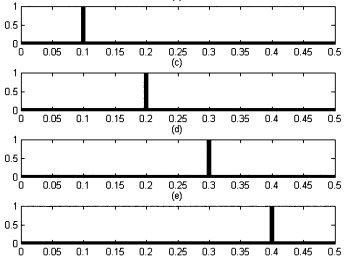
\includegraphics[width=0.9\textwidth]{Figs/2009_BackPropagationFF05}\\
    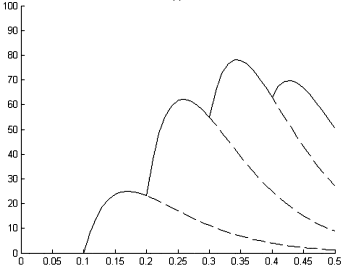
\includegraphics[width=0.9\textwidth]{Figs/2009_BackPropagationFF06}
\end{columns}
\footnotetext[1]{\fullcite{MarcoNuno_CongArbIng_2009_06_00}}
}

\frame
{
\frametitle{Arquitectura Propuesta}
\begin{columns}
    \column {0.5\textwidth}
\begin{itemize}
   \item Procesador Neural (NP) implementa las operaciones de cada neurona.
   \item Los NPs se agrupan en un módulo mas complejo, denominado Procesador de Capa de Redes Pulsantes (SNLP), que permite que cada neurona comparta una memoria donde se almacena los pesos y los retados de entrada.
   \item Los SNLP pueden instanciarse para tantas capas como sea necesario. 
   \item Existe una interfaz hacia la memoria externa y una unidad de control.
    \end{itemize}     
    \column {0.5\textwidth} 
    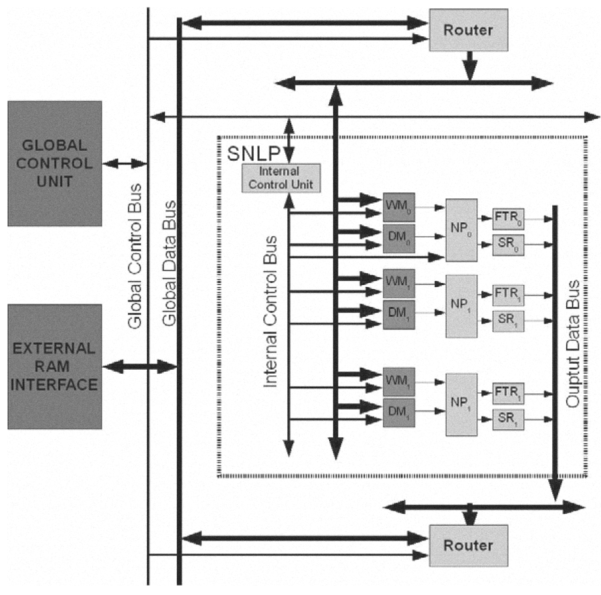
\includegraphics[width=0.9\textwidth]{Figs/2009_BackPropagationFF02}
\end{columns}
}


\frame
{
\frametitle{Arquitectura Propuesta}
\begin{columns}
    \column {0.5\textwidth}
   \begin{itemize}
   \item Un módulo de aprendizaje (LM) se encarga de hacer el ajuste de los pesos dependiendo de la tarea específica que debe ser aprendida.
   \item Un enrutador se encarga de sincronizar la transmisión de los datos entre los módulos dependiendo de la etapa de procesamiento.
   \item Existe un pipeline de $N$ etapas dependiendo del número de SNLPs que se incorporen al sistema.
    \end{itemize} 
    \column {0.5\textwidth} 
    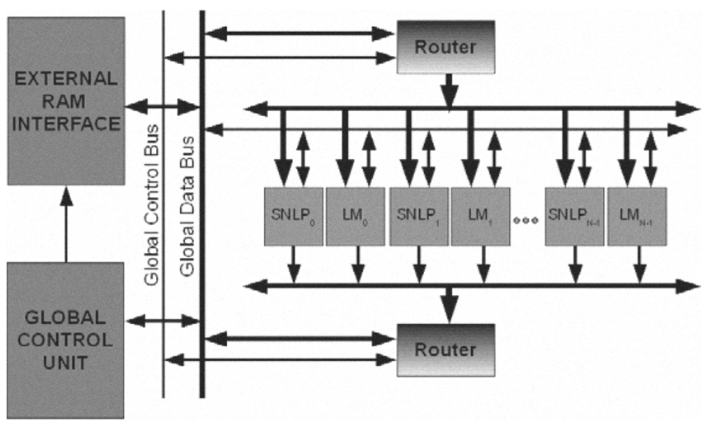
\includegraphics[width=0.9\textwidth]{Figs/2009_BackPropagationFF01}
\end{columns}
}




\frame
{
\frametitle{Resultados}
\begin{columns}
    \column {0.65\textwidth}

\begin{itemize}
\item Se probó con un conjunto de datos de 128 filas por 4 columnas generado aleatoriamente. 
\item Se obtuvó el tiempo de ejecución para diferentes topologías utilizando 2 SNLP con varios NPs (4, 8 y 16). 
\item Las topologías probadas contienen 3 capas de neuronas, y el número de neuronas por capa varía desde 64 neuronas por capa oculta y de salida hasta 256 neuronas por capa oculta y de salida.
\item Se compara el tiempo de ejecución en SW vs el tiempo de ejecución en Hardware para diferentes configuraciones. 
\end{itemize} 

    \column {0.35\textwidth} 
        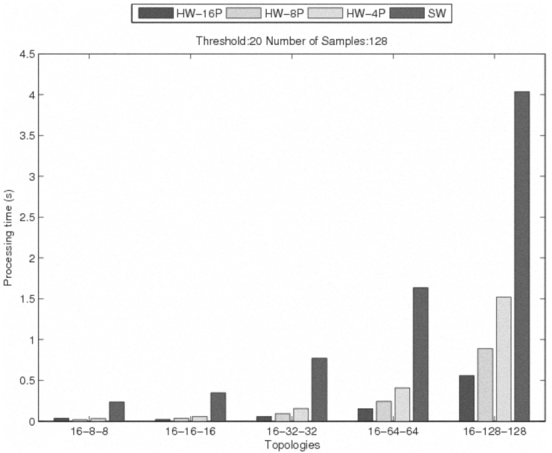
\includegraphics[width=0.9\textwidth]{Figs/2009_BackPropagationFF03}\\
        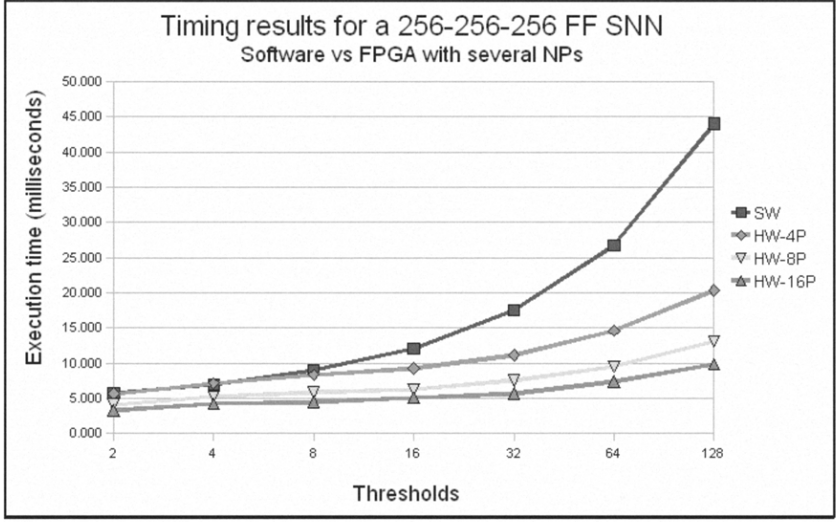
\includegraphics[width=0.9\textwidth]{Figs/2009_BackPropagationFF04}
\end{columns}
}

